\section{Constraining the tensor power spectrum}
The first analysis we conducted aims to show how data from a future PIXIE-like experiment can improve current constraints on the tensor-to-scalar ratio $r$. For this analysis we first produced a fiducial set of data using $\Lambda$CDM parameters with $r=0$, which corresponds to the absence of spectral distortions. At this point, we run four MCMC simulations fixing all the $\Lambda$CDM parameters and varying the tensor-to-scalar ratio at two different scales $k_1=0.02$ Mpc$^{-1}$ and $k_2=0.005$ Mpc$^{-1}$. In this way, we were able to constraint directly the tensor primordial power spectrum at these two scales, which approximately correspond to the bounds of the range of scales probed by CMB anisotropies. To begin with we reproduced the constraints set by BICEP/\textit{Keck} 2018 alone (red plots in Figure \ref{fig:r_const}), then we run 3 MCMC analysis combining these data with our PXIE-like experiment. In these runs we allowed for different PIXIE-foreground nuisance parameters to vary to study how they influence the constraint. In particular, we first allowed for all the foreground parameters to vary (blue plot in Figure \ref{fig:r_const}), then we fixed them all except for the y amplitude from reionization (green plot in Figure \ref{fig:r_const}) and lastly we fixed all of them (orange plot in Figure \ref{fig:r_const}). 
\begin{figure}[t]
        \centering
        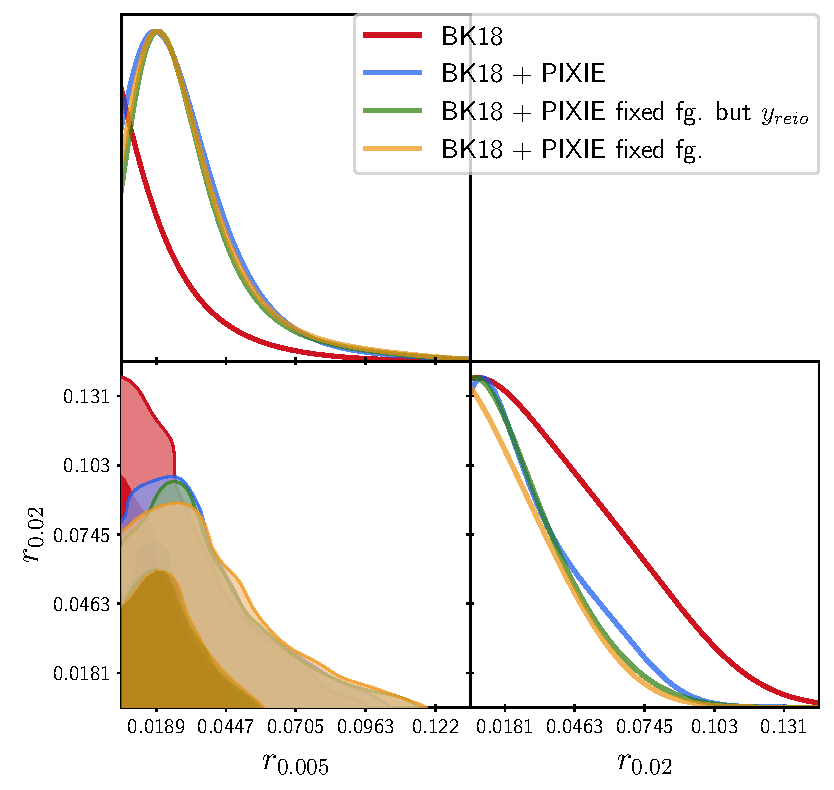
\includegraphics[width=.8\textwidth]{Constraints/BKPIXIE.pdf}
        \caption{Posterior distribution of the tensor-to-scalar ratio $r$ at two different scales. The red contour is obtained using only data from BICEP/\textit{Keck} 2018 \cite{Ade_2021} while the other contours are obtained combining BICEP/\textit{Keck} 2018 with simulated data from a PIXIE-like experiment.}
        \label{fig:r_const}        
    \end{figure}
Figure \ref{fig:r_const} shows how combining spectral distortions constraint with CMB anisotropies data improves the constraints on $r$ at both scales. Indeed, the 95\% CL upper limits $r_{0.005}<0.060$ and $r_{0.02}<0.103$, obtained only from BICEP/\textit{Keck} 2018 data, are improved to 
\begin{align*}
    &r_{0.005}<0.077,\quad &r_{0.02}<???\qquad&\text{95\%CL with foreground,}\\
    &r_{0.005}<???,\quad &r_{0.02}<\times0.067\qquad&\text{95\%CL with only $y_{\text{reio}}$,}\\
    &r_{0.005}<0.076,\quad &r_{0.02}<0.065\qquad&\text{95\%CL with fixed foreground}.
\end{align*}
This opens for the possibility of further constraining the tensor-to-scalar ratio by combining the data we used with \textit{Planck} \cite{planck2018results} data. 
\section{Constraining lognormal bumps}
In this last section we discuss the second type of constraints that we obtained. To begin with, we constrained the height of a lognormal bump placed at $k_\text{pk}=10$ Mpc$^{-1}$ using simulated data from the PIXIE experiment \cite{pixie}. We started producing a fiducial set of data from a power spectrum without the bump, then using \textbf{\texttt{MontePython}} we obtained 3 different types of constraints: the first one in which all the nuisance parameters presented in Table \ref{tab:nui_pixie}, a second one with a fixed foreground and a last one in which, by letting vary also $y_\text{reio}$, we marginalized over it.  In all the three cases we fixed the width of the bump at an intermediate value of $\sigma_\text{bump}=0.44$.\\
The analysis performed considering all the foreground nuisance parameters, shown in Figure \ref{fig:LN}, results in a constraint on the amplitude of the bump of $\mathcal{A}_\text{bump}<3.2\times10^{-2}$ at 95\% CL. This constraint becomes more stringent if we assume a perfect knowledge of the foreground parameters, as shown in Figure \ref{fig:LN_NN}, resulting in $\mathcal{A}_\text{bump}<7.7\times10^{-5}$. A milder constraint results instead if we marginalize only over $y_\text{reio}$, as shown in Figure \ref{fig:LN_NN_reio}, resulting in $\mathcal{A}_\text{bump}<4.0\times10^{-4}$.\\ 
\begin{figure}
    \centering
    \begin{subfigure}{0.49\textwidth}
        \centering
        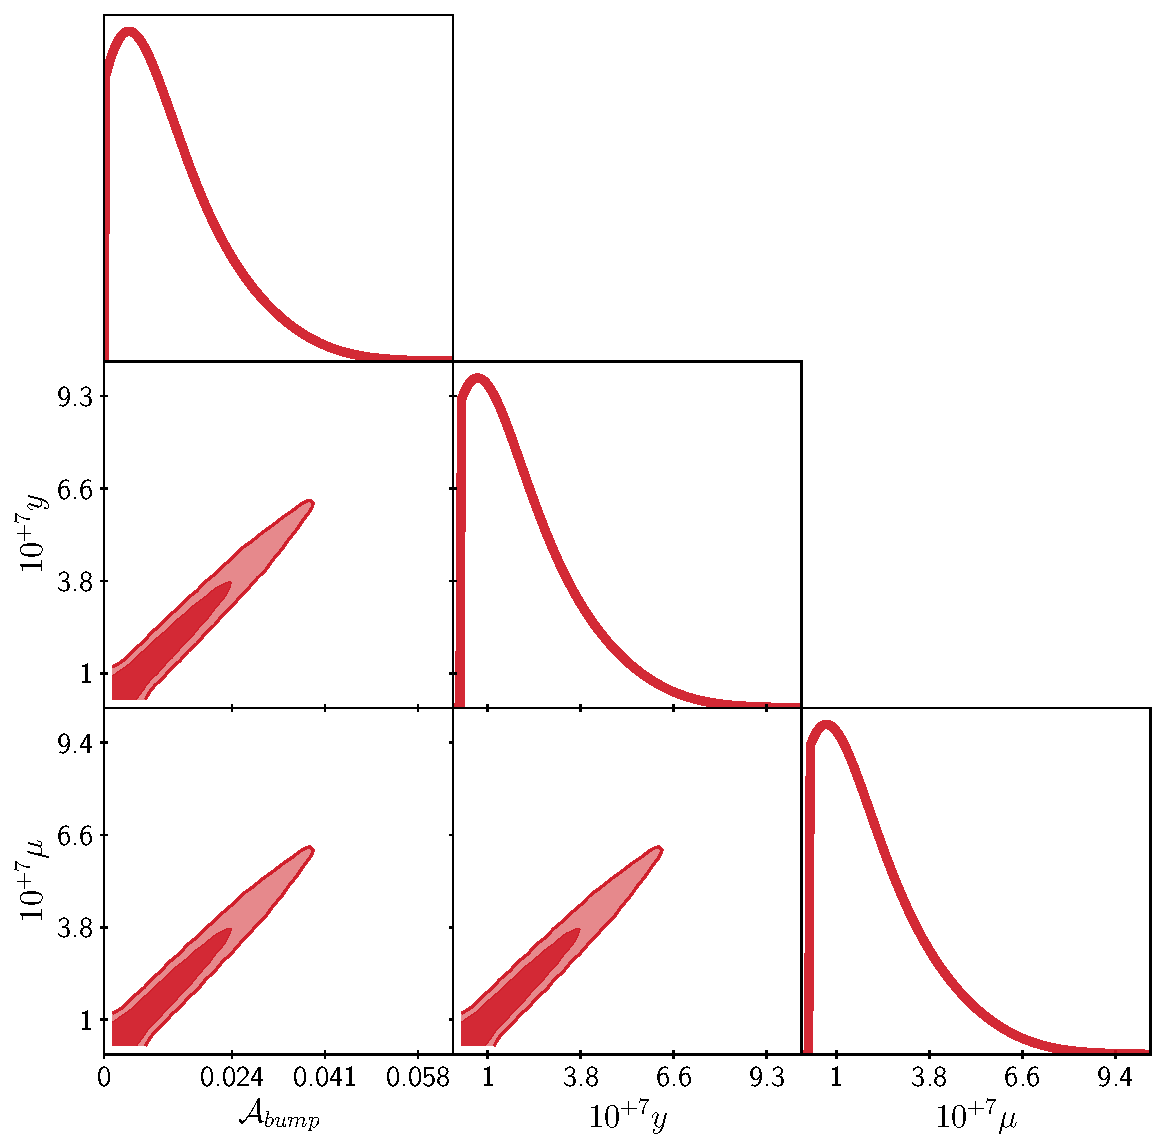
\includegraphics[width=1\textwidth]{Constraints/Lognormal.pdf}
        \caption{PIXIE with foreground}
        \label{fig:LN}        
    \end{subfigure}
    \hfill
    \begin{subfigure}{0.49\textwidth}
        \centering
        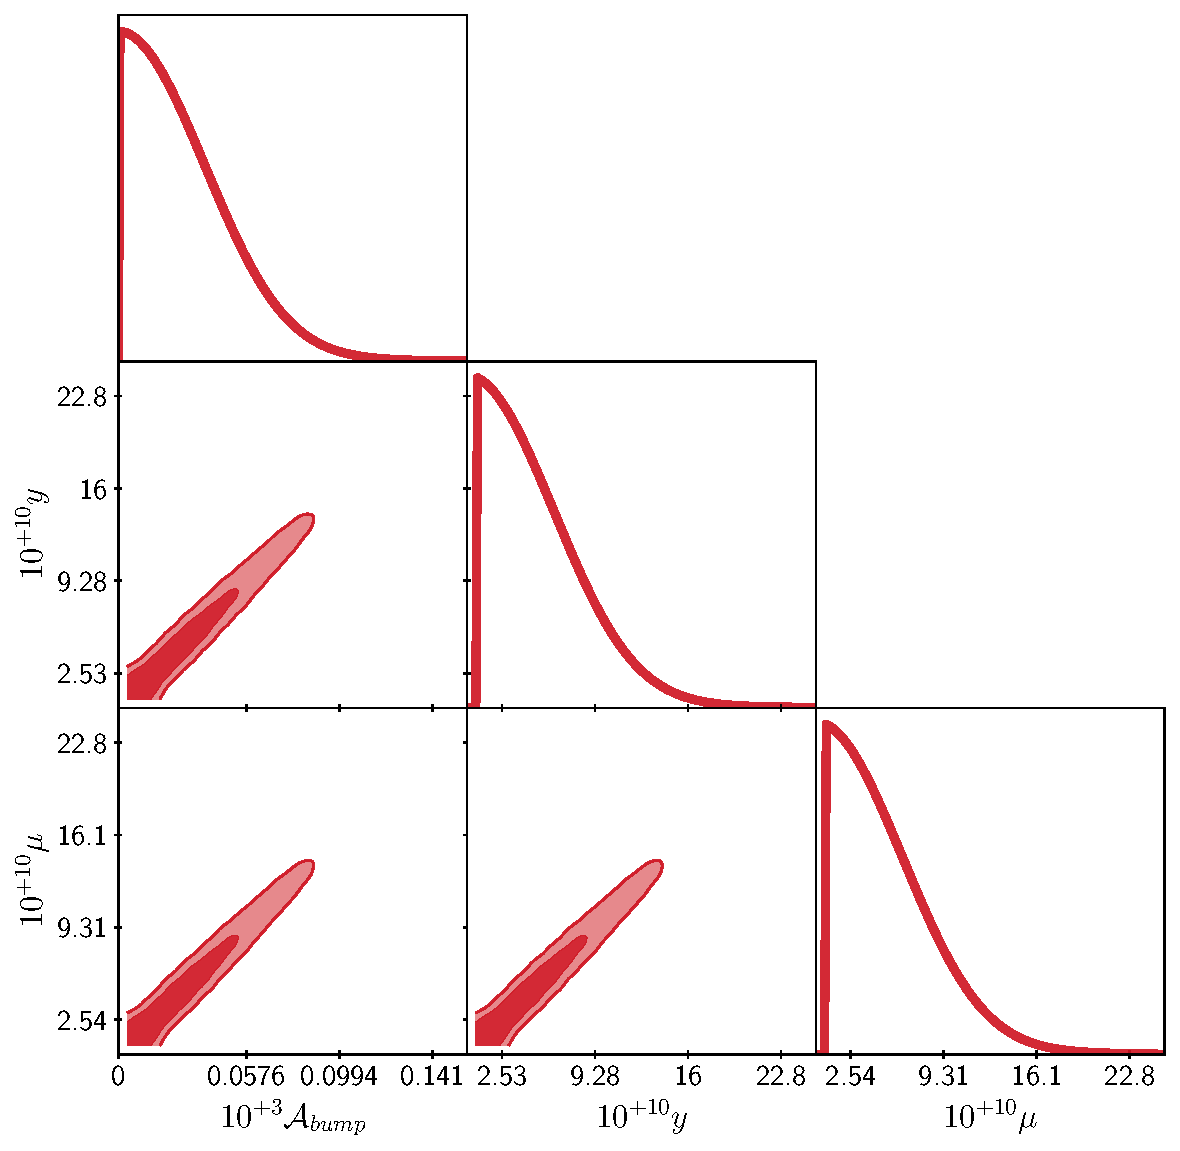
\includegraphics[width=1\textwidth]{Constraints/LN_NN.pdf}
        \caption{PIXIE without foreground}
        \label{fig:LN_NN}        
    \end{subfigure}

    \vspace{1em}

    \begin{subfigure}{0.7\textheight}
        \centering
        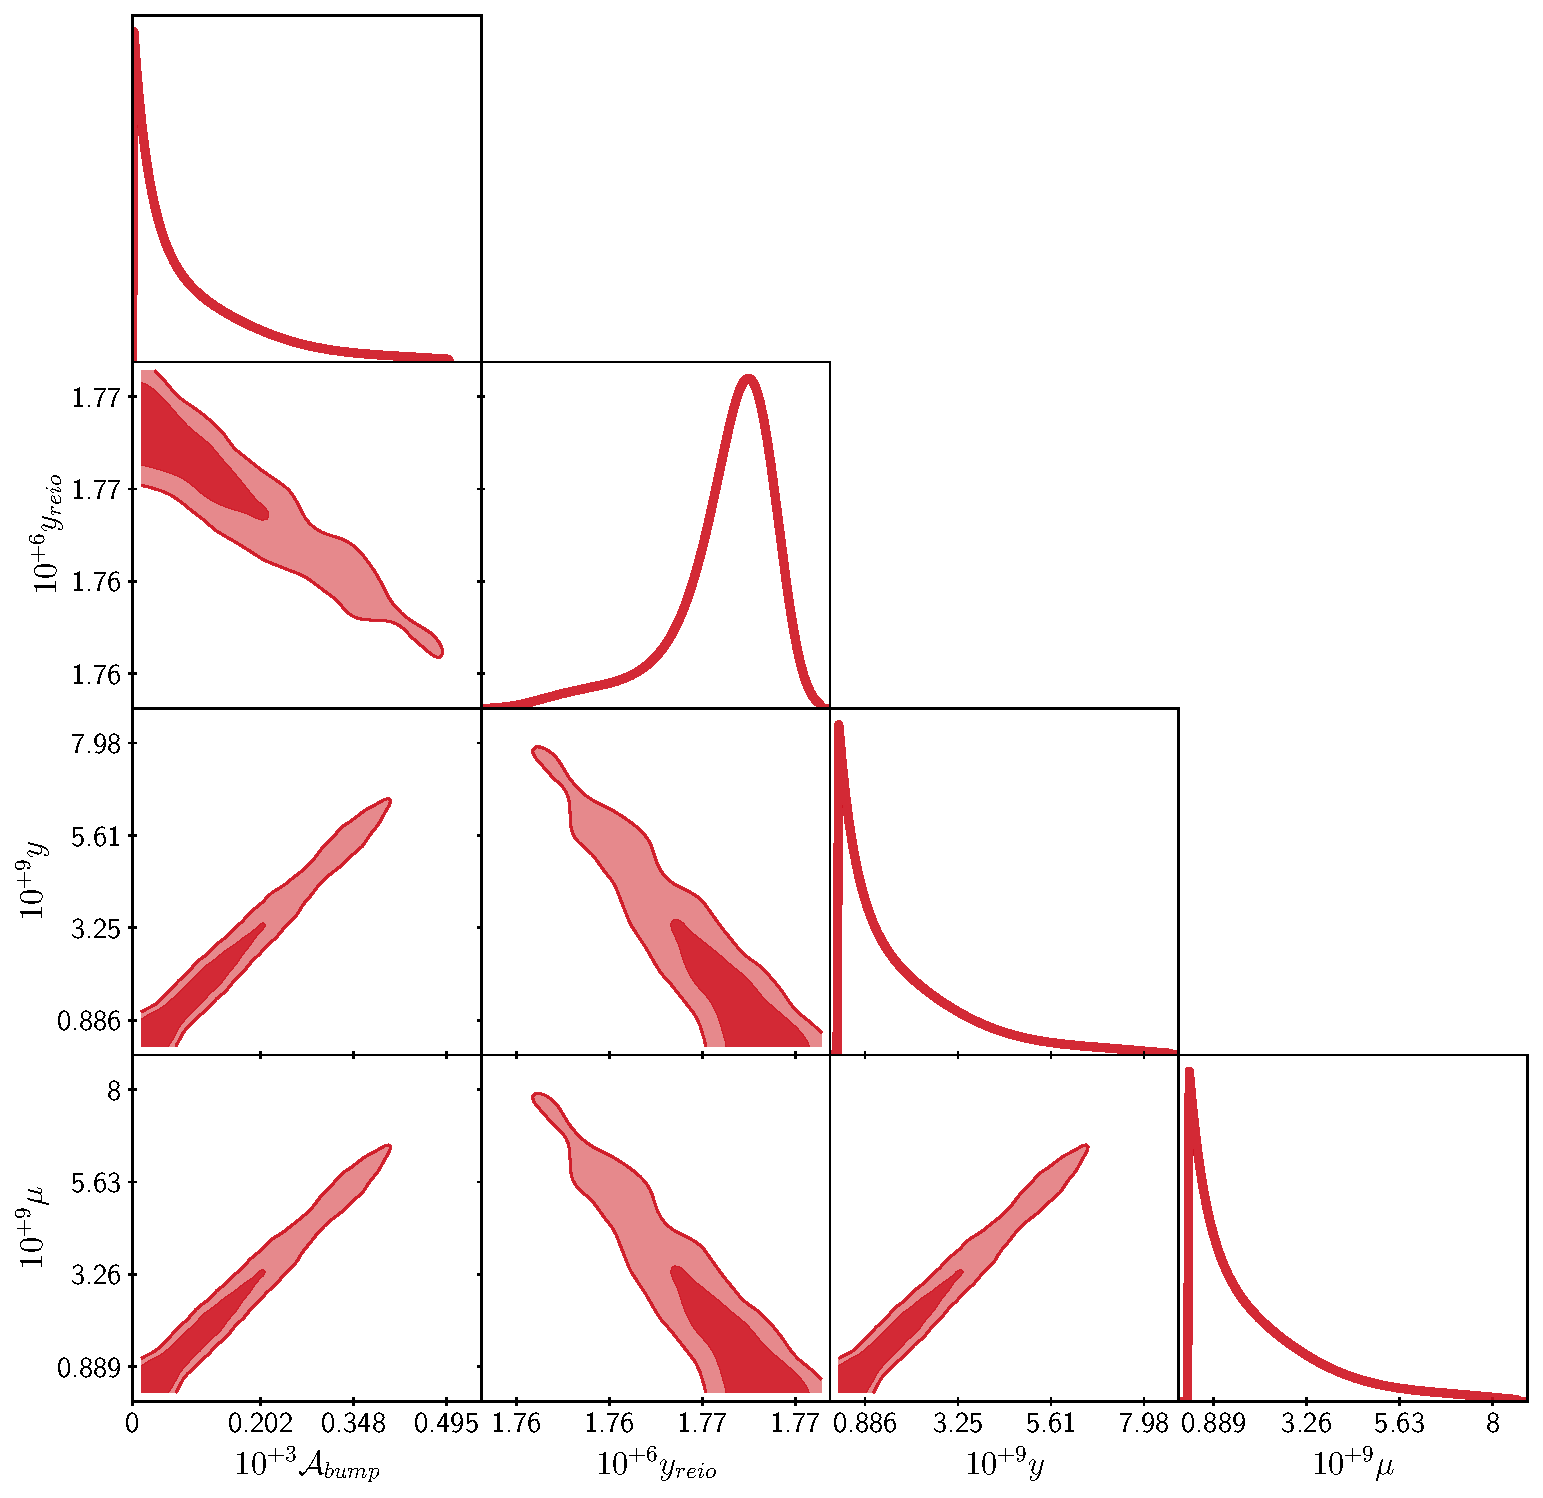
\includegraphics[width=0.5\textwidth]{Constraints/LN_NN_reio.pdf}
        \caption{PIXIE with only $y_\text{reio}$}
        \label{fig:LN_NN_reio}        
    \end{subfigure}
    \caption{Marginalized posterior distributions for the amplitude of a lognormal bump placed at $k_\text{pk}=10$ Mpc$^{-1}$ with width $\sigma_\text{bump}=0.44$. The three panels show the results obtained with different assumptions on the nuisance parameters.}
    \label{fig:LN_all}
\end{figure}



